\documentclass[crop, tikz]{standalone}

\usepackage[utf8]{inputenc}
% 'crop' is the default for v1.0, before it was 'preview'
%\usetikzlibrary{...}% tikz package already loaded by 'tikz' option

\usetikzlibrary{arrows}
\usetikzlibrary{decorations.markings}
\usetikzlibrary{patterns}
\usetikzlibrary{calc}

\begin{document}

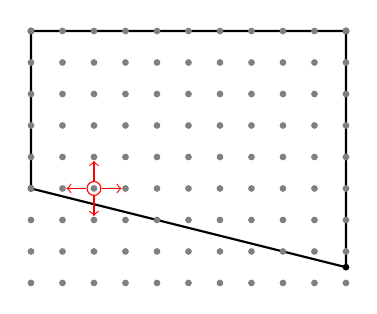
\begin{tikzpicture}
	% draw nodes
	\filldraw[black] (0,0) circle [radius=1pt];
	\filldraw[black] (0,2) circle [radius=1pt];
	\filldraw[black] (4,2) circle [radius=1pt];
	\filldraw[black] (4,-1) circle [radius=1pt];
	
	% draw region outline
	\draw[thick, black] (0,0) -- (0,2) -- (4,2) -- (4,-1) -- cycle;

	% draw uniform in each dimension mesh
	\foreach \x in {0,0.4,...,4} {
		\foreach \y in {0,0.4,...,2} {
			\filldraw[black!50!white] (\x,\y) circle [radius=1pt];
		}
		\foreach \y in {-0.4,-0.8,...,-1.3} {
			\filldraw[black!50!white] (\x,\y) circle [radius=1pt];	
		}
	}

	% draw the problem nodes
	\draw[red] (0.8,0) circle [radius=2.5pt];
	\draw[red, ->] (0.8,-0.1) -- (0.8,-0.35);
	\draw[red, ->] (0.8,0.1) -- (0.8,0.35);
	\draw[red, ->] (0.7,0) -- (0.45,0);
	\draw[red, ->] (0.9,0) -- (1.15,0);
\end{tikzpicture}

\end{document}